% Launch-Bound and Cache-Aware: Predicting VLA Inference Latency and CUDA-Graph Speedup
% Across GPU Generations. Course project, GPU Architecture and Programming, NYU, Fall 2026.
% DRAFT 2026-11-13. Numbers marked \pending{} wait for runs listed in CLAUDE.md section 0.1.
% Style rule for this paper: no em dashes.
\documentclass[10pt,twocolumn]{article}
\usepackage[margin=0.8in]{geometry}
\usepackage{graphicx,booktabs,amsmath,hyperref,xcolor}
\newcommand{\pending}[1]{\textcolor{orange}{[#1]}}

\title{Launch-Bound and Cache-Aware: Predicting VLA Inference Latency\\
and CUDA-Graph Speedup Across GPU Generations}
\author{Aditya Maddur Guruprakash\\New York University}
\date{}

\begin{document}
\maketitle

\begin{abstract}
Vision-language-action (VLA) robot policies run at batch size 1 and issue thousands of short
GPU kernels per control step. We ask the Project 2 question (flavor B): given a kernel trace of
such a workload on one GPU, can we predict its latency on another GPU? We trace SmolVLA
(450M) on three GPUs from three architecture generations (RTX 2080 Ti, TITAN V, A100) and
OpenVLA-7B on the A100, in eager PyTorch and with the denoising or decoding loop captured as a
CUDA graph. 78\% of SmolVLA's kernels run for less than 5\,$\mu$s, and in eager mode 85 to
90\% of the step is host-side framework dispatch. The graph-mode loop is bound by per-kernel
latency, not bandwidth: the A100 runs it only 11\% faster than the 2080 Ti despite 2.5$\times$
the DRAM bandwidth, and the TITAN V, with more bandwidth than the 2080 Ti, is 54\% slower. We
build a two-timeline model (host dispatch and GPU execution) whose kernel term transfers each
kernel's \emph{graph slot} with ratios measured by small PyTorch microbenchmarks on the target.
Across the six source/target pairs and seven configurations it predicts the eager step with
7.5\% MAPE, the hybrid (eager prefix plus graphed loop) step with 5.2\%, and the CUDA-graph
loop with 16\%, versus 64\% for bandwidth-ratio scaling and 86 to 98\% for the VLA-Perf roofline, and it reproduces the ordering
inversion where the TITAN V host is fastest in eager mode while its GPU is slowest under
graphs.
\end{abstract}

\section{Introduction}
Robot policies built on vision-language models (OpenVLA, $\pi_0$, SmolVLA, GR00T) are now
deployed on a wide range of GPUs, and practitioners want to know how fast a policy will run on
hardware they do not have. Public benchmarks show orderings that spec sheets do not explain:
H200 slower than H100 on OpenVLA and GR00T, an RTX PRO 6000 beating an H200 at small action
chunks, and OpenVLA plateauing near the same latency on Hopper and Ada~\cite{yotta}. The
recent analytical model VLA-Perf~\cite{vlaperf} is a per-operator roofline over spec-sheet
peaks and explicitly leaves kernel launch and runtime overheads unmodeled.

Batch-1 VLA inference sits in the opposite regime from the throughput kernels classic GPU
performance models target~\cite{hongkim,gpuperf}. Our measurements show that (i) the eager step
is dominated by host-side dispatch, about 27\,$\mu$s of CPU per kernel; (ii) once the loop is
captured as a CUDA graph, kernels are a few microseconds long and their time is set by kernel
start-up and memory latency, not bandwidth; and (iii) consequently the benefit of CUDA graphs
depends on the pairing of host CPU and GPU, not on the workload alone.

\textbf{Contributions.} (1) Traces of two VLAs across three GPU generations in eager, graph and
hybrid modes, all bit-exact against the stock models. (2) Standalone CUDA C++ kernels and a C++
replay of the traced step that runs on the CIMS machines. (3) A launch-aware latency model that
predicts eager, graph and hybrid latency and CUDA-graph speedup on a target GPU from a source
trace plus target microbenchmarks. (4) An evaluation on six source/target pairs with
percentage error per case, against spec-ratio and roofline baselines.

\section{Survey}
\textbf{Analytical GPU models.} Hong and Kim~\cite{hongkim} model memory-level and
thread-level parallelism; GPUPerf~\cite{gpuperf} extends this to identify optimization
potential; Wang, Liu and Chu~\cite{wang} predict performance under frequency scaling by
cross-benchmarking. All target kernels that fill the GPU.
\textbf{Static and program-level analysis.} Alavani, Varma and Sarkar~\cite{alavani} predict a
CUDA kernel's execution time from static features of its code, and Muller and
Hoffmann~\cite{muller} give a program logic that bounds a kernel's resource cost (divergence,
uncoalesced accesses, bank conflicts). Both reason about one kernel in isolation; in our regime
most of the step's time is outside any kernel body (dispatch, launch, node gaps).
\textbf{Cross-GPU prediction for deep learning.} Habitat~\cite{habitat} predicts DNN
training iteration time on a target GPU from a trace on a source GPU, scaling kernels by
``wave scaling'' with GPU specs and using small MLPs for a few kernel types; it targets
training kernels that occupy the GPU and does not model host dispatch or CUDA graphs.
Daydream~\cite{daydream} replays a dependency graph of CPU and GPU tasks to answer what-if
questions on one machine; our two-timeline replay is the same idea, specialized to batch-1
inference and moved across GPUs. Cycle-level simulators such as Accel-Sim~\cite{accelsim}
are accurate but orders of magnitude too slow for 13{,}000-kernel steps on many targets.
\textbf{VLA performance.} VLA-Perf~\cite{vlaperf} predicts an upper bound with
$T_o = \max(\mathrm{FLOPs}_o/P, \mathrm{Bytes}_o/B)$ per operator, validated on one platform
($\pi_0$ on an RTX 4090, 73 to 83\% fidelity). Real-time VLA work~\cite{realtime} reports about
2$\times$ from CUDA graphs on $\pi_0$, but no one predicts when graphs pay off.
\textbf{Launch overhead and CUDA graphs.} CUDA graphs~\cite{cudagraphs} record a sequence of
kernels once and replay it with one launch, removing per-kernel CPU launch cost; PyTorch
exposes them for static-shape regions~\cite{ptgraphs}. Their benefit depends on how much of
the step is CPU-side launch and framework overhead, which we measure and model directly.

\section{Problem Definition and Challenges}
Given a profiled step on a source GPU $S$ (per-kernel durations, launching ops, sync points)
and a description of a target GPU $T$, predict on $T$: the eager step latency, the latency of
the loop captured as a CUDA graph, the hybrid step (eager prefix plus graphed loop), and the
graph speedups. Challenges: (a) the eager step is host bound, so the host CPU of $T$ matters;
(b) profiling inflates each kernel by about 1\,$\mu$s, comparable to the kernels themselves;
(c) small-kernel time does not follow bandwidth or FLOP ratios; (d) different GPUs run
different cuBLAS kernels (kernel counts per step differ by about 1\%).

\section{Proposed Idea}
\textbf{Two-timeline replay.} For eager mode we replay the traced kernel sequence on a CPU and
a GPU timeline. The CPU spends $d_k = c_{\mathrm{op}(k)} + p$ on kernel $k$: the PyTorch
dispatch cost of its aten op class from a microbenchmark table, plus a Python residual $p$.
The GPU starts $k$ at $\max(\mathrm{cpu}_k, \mathrm{gpu}_{k-1} + g_{\mathrm{eager}})$ and runs
it for $t_k$; host-device copies synchronize the timelines. $g_{\mathrm{eager}}$ is a GPU-side
per-kernel cost of stream launches measured with dependent spin-kernel chains (about
2\,$\mu$s on the A100, and it does not shrink for long kernels). For graph mode,
$T_{\mathrm{graph}} = L_{\mathrm{graph}} + \sum_k (t_k + \delta_{\mathrm{node}})$.

\textbf{Two fitted parameters, on the source only.} The profiler bias $b$ (subtracted from
traced durations) and $p$ are fitted on one baseline run of the source and held fixed for all
other configurations and all targets.

\textbf{Kernel transfer by graph slots.} We transfer the slot $u_k = t_k + \delta_S$ rather
than the duration: $u_k^T = r_c \min(u_k, \tau_c) + r_{\mathrm{bw}}\max(u_k - \tau_c, 0)$,
where $r_c$ is the ratio of target to source slot time of a PyTorch microbenchmark op of the
same class (elementwise, allocating op, GEMM, attention) replayed as a CUDA graph, $\tau_c$
the source slot of that op, and $r_{\mathrm{bw}}$ the measured DRAM bandwidth ratio
(variant \emph{slot}; \emph{slot per op class} omits the tail term). Host costs on $T$ come
from $T$'s dispatch table; $p_T = p_S \cdot h$ with $h$ the host speed ratio.
\textbf{Hypotheses we tested and rejected.} (i) Small kernels on cold data: in the real loop
the GEMMs stream about 250\,MB of weights per step, so we measured small PyTorch ops over a
512\,MB tensor pool. Cold data costs about 30\% more per kernel, but almost equally on every
GPU, so cold-cache slot ratios do not improve the transfer (graph loop MAPE 22\% vs 16\%).
(ii) Host Python speed: pure-Python and \texttt{nn.Module} call benchmarks run at the same
speed on all three hosts (within 10\%), so $p$ does not scale with Python speed; the hosts
differ in the aten/C++ dispatch path, which is what $h$ measures.

\section{Experimental Setup}
\begin{table}[t]\centering\small
\begin{tabular}{lrrrr}\toprule
GPU & SMs & L2 & DRAM BW & host CPU\\\midrule
RTX 2080 Ti (cuda2) & 68 & 5.5\,MB & 582\,GB/s & Xeon E5-2660 v3\\
TITAN V (cuda3) & 80 & 4.5\,MB & 648\,GB/s & Xeon Gold 5118\\
A100-SXM4-40GB & 108 & 40\,MB & 1479\,GB/s & cloud Xeon 2.2\,GHz\\
RTX 4070 (cuda5) & 46 & 36\,MB & 475\,GB/s & Xeon E5-2650 v2\\\bottomrule
\end{tabular}
\caption{GPUs. Bandwidth measured with our sweep (bench/calib). The RTX 4070 was added after
the main analysis (Section~\ref{sec:rtx4070}); headline cross-GPU numbers use the first three.}\label{tab:gpus}
\end{table}
GPUs in Table~\ref{tab:gpus}; GTX TITAN X (Maxwell) was calibrated only. Software: PyTorch
2.10/CUDA 12.8 for SmolVLA (same build on all hosts), PyTorch 2.2/CUDA 12.1 for OpenVLA; our
CUDA code builds with nvcc 12.4. Workloads: SmolVLA in FP16, 1 to 3 cameras, 5/10/20 flow
steps, action chunk 25/50/100; OpenVLA-7B in FP16 with one image and 7 action tokens.
Timing: CUDA events or host timers after warm-up, \texttt{CUDA\_MODULE\_LOADING=EAGER},
medians of 20 or more repetitions, idle GPUs (checked before every stage on the shared CIMS
machines). Traces use the PyTorch profiler (CUPTI).

\section{Experiments and Analysis}
\subsection{Where the time goes}
SmolVLA on the A100: eager step 377\,ms, of which the GPU is busy 58\,ms; 13{,}190 kernels
per step, median 3.3\,$\mu$s. Capturing the 10-step denoising loop as a CUDA graph cuts it
from 316 to 35.8\,ms (8.8$\times$), and the step from 377 to 94\,ms (4.0$\times$). OpenVLA:
decode is 40\,ms per token eager, 14.2\,ms as a graph (62\% of the weight-streaming bound),
2.0$\times$ end to end. Our C++ replay of SmolVLA's loop runs eager in 44.7\,ms on the 2080
Ti versus 407\,ms in PyTorch, so about 89\% of eager time is framework dispatch.

\subsection{Small kernels are latency bound}
Matching identical PyTorch kernels across GPUs, kernels below 6\,$\mu$s take the same time on
the A100 and the 2080 Ti (ratio 0.98 to 1.02) and 1.3 to 1.5$\times$ longer on the TITAN V.
Profiling adds the same 11.3\,ms (about 0.95\,$\mu$s per kernel) to a graph replay on all
three GPUs. Real graph slots per kernel are 3.0, 3.4 and 5.2\,$\mu$s on the A100, 2080 Ti
and TITAN V.

\subsection{Same-GPU accuracy}
Fitted on one A100 run per model, held-out MAPE: SmolVLA eager 1.8\%, graph loop 0.7\%,
hybrid 2.8\%; OpenVLA eager 0.7\%, graph decode 0.3\%. Summing kernel times (what a roofline
model predicts at best) errs by 84\% on the eager step and 24\% on the graph loop.

\subsection{Cross-GPU accuracy}
\begin{figure*}[t]\centering
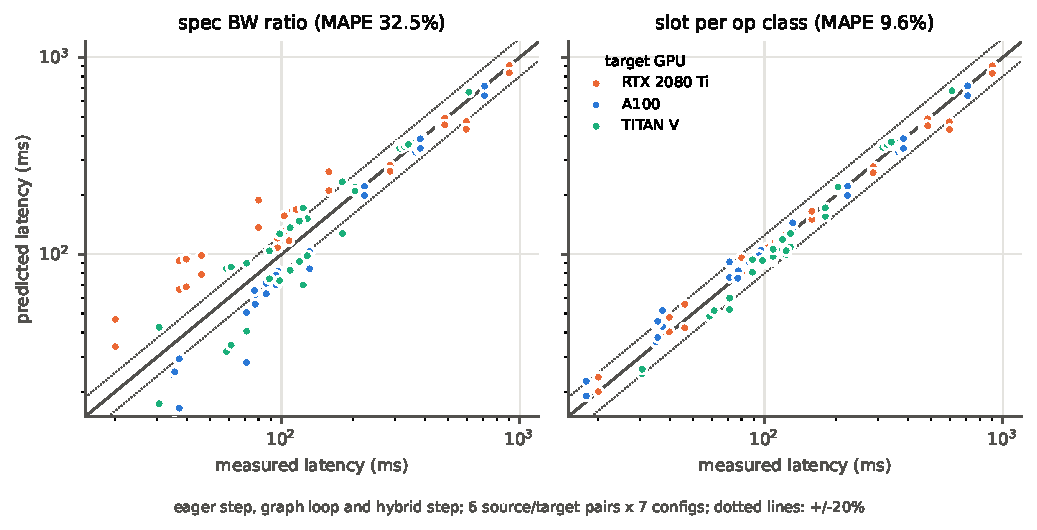
\includegraphics[width=0.62\textwidth]{figures/pred_vs_meas.pdf}
\caption{Predicted vs measured latency on the target GPU (6 pairs $\times$ 7 configs).}
\label{fig:pvm}
\end{figure*}
\begin{figure*}[t]\centering
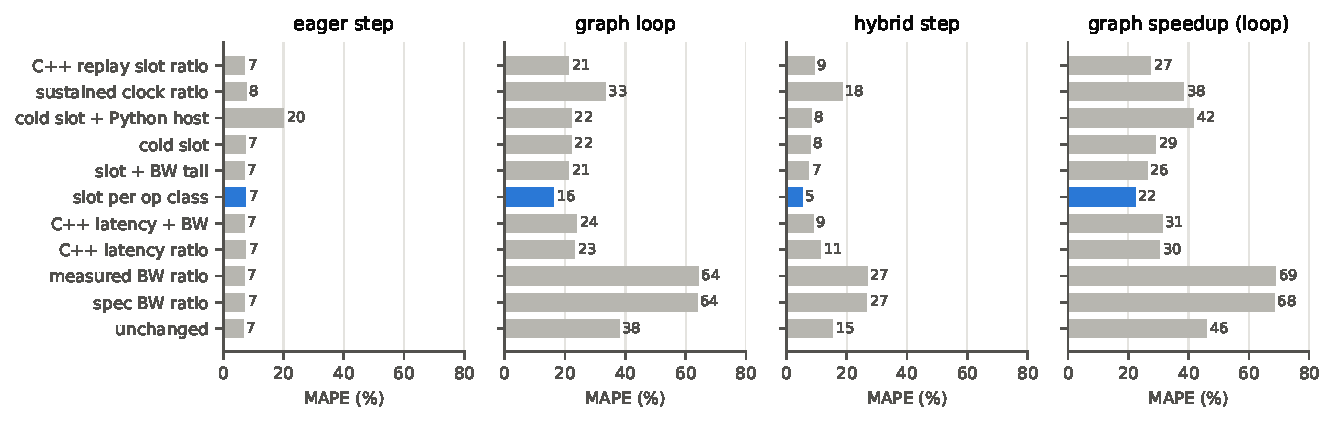
\includegraphics[width=\textwidth]{figures/mape_variants.pdf}
\caption{Cross-GPU MAPE by kernel-transfer variant.}\label{fig:mape}
\end{figure*}
Figures~\ref{fig:pvm} and~\ref{fig:mape}. With slot ratios per op class the MAPE is 7.5\%
(eager), 5.2\% (hybrid), 16\% (graph loop) and 22\% (loop graph speedup); bandwidth-ratio
scaling gives 64\% on the graph loop. Between the 2080 Ti and the A100 every quantity is within
6\%. Pairs with the TITAN V are worst (graph loop 17 to 29\%): the hot-cache microbenchmarks
see a 1.2 to 1.5$\times$ slot ratio where the real loop has 1.54$\times$.
The missing factor is the \emph{sustained} SM clock. Sampling \texttt{nvidia-smi} while
the C++ replay of the loop runs shows the TITAN V holding 1335\,MHz (spec maximum 1912) and
the 2080 Ti 1950\,MHz; the ratio, 1.46, matches the real per-kernel ratio of 1.54. Scaling all
slots by the sustained-clock ratio predicts the graph loop between these two GPUs within 6 to
7\% in both directions (versus 17 to 22\% with slot ratios), so latency-bound kernels scale
with the clock the GPU actually runs at, not its spec boost clock. The clock alone does not
transfer across architectures, though: the A100 sustains only 1410\,MHz, below the 2080 Ti,
yet runs small kernels in the same time, and clock-only scaling over all six pairs gives 33\%
MAPE on the graph loop. Per-op-class slot ratios measured on the target capture both the
architecture and the clock it runs at, which is why they are our default; a target's
sustained clock is a cheap extra feature when source and target share an SM design.

\subsection{How much does L2 residency matter?}
To isolate the cache term we rerun our C++ replay of the 10-step loop with all GEMM weights
sharing a pool of $N$ MB, so the loop touches $N$ MB of distinct weights with unchanged shapes
and kernels, and sweep $N$ from 3 to 256\,MB. On the A100 (40\,MB L2, about 20 to 27\,MB
effective in our bandwidth sweep) the graphed loop takes 31.2\,ms when the weights fit in L2 and
32.2\,ms when they stream from DRAM with cuBLAS GEMMs (3\%), and 43.5 vs 49.6\,ms with our own
GEMM (12\%), with the knee between 16 and 24\,MB. The saving is bounded by the DRAM time of the
weights: 250\,MB per denoising step at 1.48\,TB/s is about 1.7\,ms of a 32\,ms loop, while the
rest is per-kernel latency. On the 2080 Ti, flushing L2 before every kernel costs 18\% (Nsight
Compute). So for small VLAs the cache term is second order next to launch and per-kernel
latency, which is why our model does without one. The same sweep on the CIMS GPUs puts each
knee at that GPU's L2 (4 to 8\,MB on the 2080 Ti and TITAN V, 24 to 48\,MB on the RTX 4070) and
bounds the saving at 6.3\%, 3.0\% and 9.1\% with cuBLAS (5.1\%, 1.0\% and 12.8\% with our
GEMM). The RTX 4070, with the largest L2 relative to its bandwidth, gains most, but the real
expert's 250\,MB of weights per step exceed every L2 we measured, so in the actual loop they
stream from DRAM on all four GPUs.

\subsection{Comparison with VLA-Perf}
\begin{table}[t]\centering\small
\begin{tabular}{lrr}\toprule
Quantity (SmolVLA) & VLA-Perf & Ours (cross-GPU)\\\midrule
Eager step & 97.7 & 7.5\\
Eager prefix & 90.1 & 8.6\\
Graph loop & 93.2 & 16.2\\
Hybrid step & 91.5 & 5.2\\
Graph speedup (loop) & 85.8 & 22.3\\\bottomrule
\end{tabular}
\caption{MAPE (\%) of VLA-Perf, run on the same models and GPUs, vs our model. VLA-Perf uses
spec sheets only; ours uses a source trace plus target microbenchmarks.}\label{tab:vlaperf}
\end{table}
We ran VLA-Perf's code~\cite{vlaperf} on our workloads: SmolVLA component configurations
matching \texttt{smolvla\_base} as traced (vision prefill per camera, VLM prefill over the
prefix, flow steps $\times$ action-expert parallel decode, as in its $\pi_0$ pipeline), and its
own OpenVLA model with our prefix length, at batch 1 on one GPU in FP16, with spec-sheet
entries for the 2080 Ti and TITAN V in its own convention. It predicts 3.9\,ms for a SmolVLA
step on the A100, against 383\,ms measured eager, 95\,ms hybrid and 35.6\,ms for the graph loop
alone; its expert time (1.5\,ms for 10 passes) is exactly the time to stream the expert's
weights at peak bandwidth, a correct roofline. For OpenVLA on the A100 it predicts 68\,ms vs
311\,ms eager and 47\,ms vs 85\,ms for the graphed decode, closer because OpenVLA's decode
GEMVs are bandwidth bound. Table~\ref{tab:vlaperf} summarizes: VLA-Perf errs by 86 to 98\% on
SmolVLA, and its GPU ordering (A100, TITAN V, 2080 Ti, by peak FLOP/s) matches neither the
measured eager ordering (TITAN V, A100, 2080 Ti) nor the graph ordering (A100, 2080 Ti, TITAN V).
This is not a flaw in its arithmetic: it is designed as an achievable upper bound. It shows
that for small batch-1 VLAs the gap between that bound and reality is one to two orders of
magnitude, and that the gap is launch, dispatch and per-kernel latency, which it does not model.

\subsection{Ordering inversion}
Measured eager step: TITAN V 340\,ms $<$ A100 383 $<$ 2080 Ti 484; graph loop: A100 35.6 $<$
2080 Ti 39.8 $<$ TITAN V 61.4. The model reproduces both orderings from every source GPU;
bandwidth scaling never does. Graph speedup is therefore a property of the host-GPU pair:
10.2$\times$ on cuda2, 9.0$\times$ on the A100 node and 4.6$\times$ on cuda3.

\subsection{A fourth GPU: RTX 4070 behind an older host}\label{sec:rtx4070}
The RTX 4070 (Ada, 36\,MB L2, 475\,GB/s measured, 2760\,MHz sustained under the workload)
sits on cuda5, whose 2013 Xeon E5-2650 v2 dispatches PyTorch ops 1.5 to 2.7$\times$ slower than
the other hosts (an eager add costs 17.4 vs 7.0 to 8.2\,$\mu$s) and runs Python 1.2 to
1.4$\times$ slower. It gives the most extreme inversion we measured: the slowest eager step of
the four GPUs (607\,ms) and the fastest graph loop (22.8\,ms, faster than the A100's
35.6\,ms), so its loop graph speedup is 22.5$\times$ versus 4.6 to 10.2$\times$ elsewhere.
Nsight Compute on the C++ flow step shows the larger L2 at work: warm-cache DRAM traffic per
flow step is 271\,MB versus 408\,MB on the 2080 Ti, and flushing L2 before every kernel costs
28\% versus 18\%.

With the 4070 as an unseen target, the graph loop transfers well (\texttt{slot\_class}: 10\%
from the 2080 Ti, 9\% from the A100, and 5 to 6\% in the other direction), but the eager step
does not: predictions into the 4070 are 41 to 60\% too high. The model scales all host time by
the target's aten dispatch ratio (2.0 to 2.6$\times$ here), while the measured eager step is
only 1.25 to 1.8$\times$ slower than on the other hosts; the Python share of the step scales
more like host Python speed (scaling it that way gives $-2$ to $+21\%$ for the 4070, but is
worse among the first three GPUs). Over all four GPUs, \texttt{slot\_class} gives 24\%
(eager), 15\% (graph loop) and 15\% (hybrid) MAPE. How to transfer the Python share between
very different hosts is the main open problem the fourth GPU exposes.

\section{Conclusions}
For batch-1 VLA inference, latency prediction across GPUs is a launch and latency problem
before it is a bandwidth or FLOP problem. A model that replays the host and GPU timelines,
corrects profiler bias, and transfers per-kernel graph slots with a handful of target
microbenchmarks predicts eager and hybrid latency within about 5 to 8\%, and reproduces
orderings that spec ratios get wrong. Limitations: one host per GPU, SmolVLA only for
cross-GPU validation, and an eager host model that does not transfer to a much slower host
(the RTX 4070 on cuda5, Section~\ref{sec:rtx4070}), although the graph loop does. The largest
L2 we could measure is 40\,MB, so the PRO 6000 (128\,MB) inversion remains untested.

\begin{thebibliography}{9}
\bibitem{vlaperf} W.~Jiang, J.~Clemons, K.~Sankaralingam, C.~Kozyrakis. How Fast Can I Run My
VLA? Demystifying VLA Inference Performance with VLA-Perf. arXiv:2602.18397, 2026.
\bibitem{yotta} Yotta Labs. VLA inference GPU benchmarks, 2026.
\url{https://www.yottalabs.ai/post/vla-inference-gpu-benchmarks}
\bibitem{hongkim} S.~Hong, H.~Kim. An Analytical Model for a GPU Architecture with
Memory-level and Thread-level Parallelism Awareness. ISCA 2009.
\bibitem{gpuperf} J.~Sim, A.~Dasgupta, H.~Kim, R.~Vuduc. A Performance Analysis Framework for
Identifying Potential Benefits in GPGPU Applications. PPoPP 2012.
\bibitem{wang} Q.~Wang, C.~Liu, X.~Chu. GPGPU Performance Estimation for Frequency Scaling
Using Cross-Benchmarking.
\bibitem{realtime} Ma et al. Running VLAs at Real-time Speed. 2025.
% TODO verify bibliographic details of the entries below before submission.
\bibitem{alavani} G.~Alavani, K.~Varma, S.~Sarkar. Predicting Execution Time of CUDA Kernel
Using Static Analysis. IEEE ISPA/IUCC/BDCloud 2018. doi:10.1109/BDCloud.2018.00139
\bibitem{muller} S.~K.~Muller, J.~Hoffmann. Modeling and Analyzing Evaluation Cost of CUDA
Kernels. ACM Transactions on Parallel Computing, 2024. doi:10.1145/3639403
\bibitem{habitat} G.~X.~Yu, Y.~Gao, P.~Golikov, G.~Pekhimenko. Habitat: A Runtime-Based
Computational Performance Predictor for Deep Neural Network Training. USENIX ATC 2021.
\bibitem{daydream} H.~Zhu, A.~Phanishayee, G.~Pekhimenko. Daydream: Accurately Estimating the
Efficacy of Optimizations for DNN Training. USENIX ATC 2020.
\bibitem{accelsim} M.~Khairy, Z.~Shen, T.~M.~Aamodt, T.~G.~Rogers. Accel-Sim: An Extensible
Simulation Framework for Validated GPU Modeling. ISCA 2020.
\bibitem{cudagraphs} A.~Gray. Getting Started with CUDA Graphs. NVIDIA Technical Blog, 2019.
\bibitem{ptgraphs} PyTorch team and NVIDIA. Accelerating PyTorch with CUDA Graphs. PyTorch
Blog, 2021.
\end{thebibliography}
\end{document}
